\documentclass[document.tex]{subfiles}
\begin{document}
\chapter{Result and Performance Analysis}
\section{Introduction} Result analysis and performance evaluation are the main focus of a system. It's also the main target of our system PWPS to increase the accuracy and show a good performance. In this chapter, we described about the evaluation matrices those are used for performance evaluation, result and performance of PWPS.
\section{Evaluation Matrices} In our work, well-defined metrics are used to measure the performance of our system.
\subsection{Accuracy (Acc)} Accuracy (Acc) is the ratio of a total number of correctly classified samples (C) and the total number of samples (N). It varies between 0 (least accurate) and 1 (most accurate). If the accuracy is 1 that means the predictor is best. \noindent For calculating the performance of our system, we applied 5-fold cross-validation. For calculating the accuracy of our system, we use Equation \ref{eq:acc}.
\begin{equation}
Acc = {C \over N}
\label{eq:acc}
\end{equation}

\section{Result}

Figure \ref{fig:accvsalpha} shows the accuracy with respect to several values for $\alpha$ and $\beta$ in Equation \ref{eq:main}. In horizontal axes the values of $\alpha$ and in vertical axes it shows the accuracy (\%).
\begin{figure}[H]
	\begin{center}
	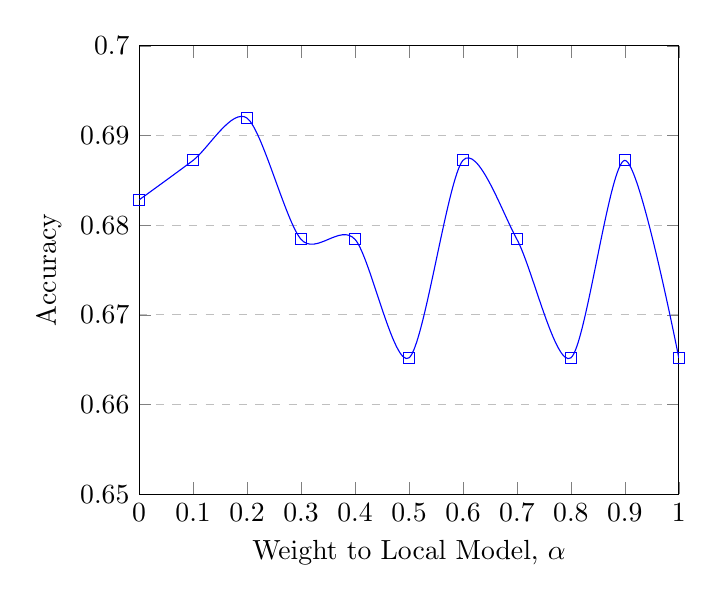
\begin{tikzpicture}
	\begin{axis}[
	%title={},
	xlabel={Weight to Local Model, $\alpha$ },
	ylabel={Accuracy},
	xmin=0, xmax=1,
	ymin=0.65, ymax=0.70,
	xtick={0.0, 0.1,0.2,0.3,0.4,0.5,0.6,0.7, 0.8, 0.9, 1.0},
	ytick={0.65, 0.66, 0.67, 0.68,0.69, 0.70},
	legend pos=north west,
	ymajorgrids=true,
	grid style=dashed,
	]
	
	\addplot[
	blue,
	mark=square,
	smooth,
	]
	coordinates {
		(0.0, 0.6828193832599119)
		(0.1, 0.6872246696035242)
		(0.2, 0.6919299559471366)
		(0.3, 0.6784140969162996)
		(0.4, 0.6784140969162996)
		(0.5, 0.6651982378854625)
		(0.6, 0.6872246696035242)
		(0.7, 0.6784140969162996)
		(0.8, 0.6651982378854625)
		(0.9, 0.6872246696035242)
		(1.0, 0.6651982378854625)
	};
	%		\legend{CuSO$_4\cdot$5H$_2$O}
	
	\end{axis}
	\end{tikzpicture}
	\end{center}
	\caption{Accuracy Versus $\alpha$}
	\label{fig:accvsalpha}
\end{figure}

In our dataset, a total number of problems is \textit{185}, and our system could solve problems \textit{128} correctly. Based on this, the accuracy of our system is \textbf{69.19\%}. Figure \ref{fig:accvsalpha} show the accuracy for different values of $\alpha$. In reverse that is also for $\beta$. The values in horizontal axes represents the value for $\alpha$ and the values in vertical axes represents the accuracy based on that. We have seen that the accuracy sometimes increases and sometime decreased based on $\alpha$. We have changed the value of $\alpha$ by \textit{0.1} and for $\alpha=0.2$ where $\beta = 1 – 0.2 = 0.8$ is the optimal value for Equation \ref{eq:main} and the accuracy is maximized.

\subsection{Comparison}
For a problem text in inference, a grounded base \textit{qsets} are formed. Then equation trees are generated by Integer Linear Programming. Finally, the based candidate equation tree is selected based on the local and the global model score. In previous, \textsc{Alges} uses the multiplies the scores of the local and the global model to get the final score as in Equation \eqref{eq:alges}.
\begin{equation}
p(t|p) \propto (\prod_{t_j \in t} \mathcal{L}_{local}(t_j|p) \times \mathcal{G}_{global}(t|p))
\label{eq:alges}
\end{equation}
In the ablation study, \textsc{Alges} have shown that the contribution of global model is superior to score of the local model. From this, in \textsc{Pwps} we have introduced the weight based method as in \eqref{eq:pwps}.
\begin{equation}
p(t|p) \propto( (\alpha  \times \prod_{t_j \in t} \mathcal{L}_{local}(t_j | p)) +( \beta \times \mathcal{G}_{global}(t|p)))
\label{eq:pwps}
\end{equation}
Where, $\alpha $ is the weight to the score of \textit{local qset relationship model} and $\beta = (1 - \alpha) $ is the weight to the score of the \textit{global equation} model.
From Figure \ref{fig:accvsalpha}, we can see that our system’s performance is high for $\alpha = 0.2$ and $\beta  = (1 – 0.2) = 0.8$.
\begin{table}[H]
	\caption{Comparison Between scoring based on equation of PWPS and ALGES}
	\begin{center}
		\begin{tabular}{|l|l|}
			\hline
			Equation of System & Accuracy (\%)\\
			\hline
			PWPS & \textbf{69.19}\\
			ALGES & 67.84\\
			\hline
		\end{tabular}
	\end{center}
	\label{tab:comp}
\end{table}


Table \ref{tab:comp} shows that the accuracy of \textbf{PWPS} is \textbf{69.19\%} which is better than the score using ALGES’s equation.

\subsection{Ablation Study}
In order to determine the effect of various components of our system on its overall performance, we perform the following ablations:
\subsubsection{No Local Model}
We test our system without a local model for generating the equations. Moreover, it is only based on Global Model. So, $\alpha = 0.0$ and $\beta = 1.0$. Without Local Model Equation \ref{eq:main} is like below:
\begin{equation}
	p(t|p) = (\beta * \mathcal{G}_{global}(t|p))
	\label{eq:Noloc}
\end{equation}
\subsubsection{No Global Model}
Here, we test our system without the global model for generating the equations which are based on the all local score of the equation. For $\alpha = 1.0$ and $\beta = 0.0$ equation without Global Model \ref{eq:main} is like below:
\begin{equation}
	p(t|p) = (\alpha * \prod_{t_i \in t} \mathcal{L}_{local}(t_i | p) ) 
	\label{eq:noGlob}
\end{equation}

Table \ref{tab:ablation} shows the result of ablation study of our system. Accuracy of PWPS is better than the No Local Model and No Global Model system.
\begin{table}[H]
	\caption{Ablation Study of PWPS}
	\begin{center}
		\begin{tabular}{|l|l|}
			\hline
			Method & Accuracy (\%)\\
			\hline
			PWPS & \textbf{69.19}\\
			No Local Model & 68.28\\
			No Global Model & 66.52\\
			\hline
		\end{tabular}
	\end{center}
	\label{tab:ablation}
\end{table}
Table \ref{tab:ablation} shows the result of ablation study of our system. Accuracy of \textbf{PWPS} is better than the No Local Model and No Global Model system.
\section{Error Analysis}
Parsing errors cause a wrong grounding into the
designed representation. For example, the parser
treats ‘regular’ as a noun modified by the number
‘13’, leading our system to treat ‘regular’ as the entity of a Qset rather than ‘Coffee’. Despite the
improvements that come from PWPS , a portion of
errors are attributed to grounding and ordering issues. For instance, the system fails to correctly distinguish between the sets of wheels, and so does not get the movement-triggering container relationships right. Semantic limitations are another source of errors. For example, PWPS does not model the semantics of ‘three consecutive numbers’. 
\begin{table}[H]
	\caption{Error in PWPS}
	\begin{center}
		\begin{tabular}{|l|l|}
			\hline
			Error Type & Problem Text (\%)\\
			\hline
			Parsing Issues& Kira’s Cafe has regular coffee and decaffeinated coffee. This  \\
			&morning, the cafe served \underline{\textit{13} regular} coffees and \underline{\textit{39} decaffeinated}\\
			& coffees. What percentage of the coffees served were regular?\\
			\hline
			Grounding Issues & There are \underline{24 bicycles} and \underline{14 tricycles} in the storage at Danny’s\\
			& apartment building. Each bicycle has 2 wheels and each tricycle \\
			&has 3 wheels. What percentage of wheels are there in bicycle?\\
			\hline
		\end{tabular}
	\end{center}
	\label{tab:grounding}
\end{table}
Finally, \textbf{PWPS} is not able to infer quantities when they are not explicitly mentioned in the text. 
\section{Conclusion} In this chapter, we have showed the result, comparison and ablation study of our system PWPS. It can conclude that our system is able to solve a reasonable number of problems.
\end{document}
